% ======================================================================
%  RAPPORT SY32 - Detection de panneaux de signalisation
%  Fichier LaTeX. Pour compiler : pdflatex -interaction=nonstopmode rapport.tex
%  Les figures sont dans ../figures/ (genere par : python src/figures.py
%  puis "python src/figures.py pr" pour la courbe precision/rappel).
%  Style volontairement sobre (classe article).
% ======================================================================
\documentclass[a4paper,10pt]{article}

\usepackage[utf8]{inputenc}
\usepackage[T1]{fontenc}
\usepackage[french]{babel}
\usepackage[margin=2.2cm]{geometry}
\usepackage{graphicx}
% Ce fichier est dans docs/ et les figures a la racine du depot (figures/) :
% on remonte d'un niveau pour resoudre les chemins includegraphics.
\graphicspath{{../}}
\usepackage{booktabs}
\usepackage{amsmath}
\usepackage{enumitem}
\usepackage{subcaption}
\usepackage[hidelinks]{hyperref}

\setlength{\parskip}{0.4em}
\setlength{\parindent}{0pt}

\title{\textbf{Détection de panneaux de signalisation routière\\par méthodes classiques}}
\author{Groupe C --- SY32 (P2026)\\
\textit{Université de technologie de Compiègne}}
\date{Juin 2026}

\begin{document}
\maketitle

\begin{abstract}
Nous présentons un programme qui retrouve les panneaux de signalisation dans une
image et entoure chacun d'une boîte accompagnée d'un score de confiance, en
n'utilisant que des méthodes classiques (l'apprentissage profond est interdit).
Le fil conducteur de notre travail tient en une phrase : \emph{on ne peut améliorer
que ce qu'on sait mesurer}. Nous avons donc d'abord construit de quoi évaluer
honnêtement le détecteur (des métriques et un jeu de validation), puis amélioré la
chaîne étape par étape, en gardant chaque idée seulement si les chiffres la
confirmaient. La détection repose sur une fenêtre glissante multi-échelle, un
descripteur \textbf{HOG + couleur + texture} et un \textbf{Random Forest}, complétés
par du \emph{hard negative mining}, un pré-filtrage couleur et une suppression des
non-maxima. Sur notre validation, l'\textit{Average Precision} est passée de
$0{,}095$ à $0{,}293$, surtout grâce à un meilleur découpage des exemples et au hard
negative mining. La première soumission sur le serveur d'évaluation a aussi révélé un
défaut majeur — une précision très basse due à un excès de fausses détections — que
nous analysons et corrigeons en fin de rapport.
\end{abstract}

% ----------------------------------------------------------------------
\section{Introduction}
% ----------------------------------------------------------------------
Le but est de détecter les panneaux dans des photos de rue : pour chaque image, le
programme doit produire une ou plusieurs boîtes englobantes, chacune avec un score
indiquant à quel point il « croit » qu'il s'agit d'un panneau. La règle imposée est
de n'employer que des méthodes classiques de vision et d'apprentissage
(\texttt{scikit-learn}, \texttt{scikit-image}, OpenCV), sans réseau de neurones
profond.

Une difficulté supplémentaire est annoncée : le jeu de test, fourni seulement en fin
de projet et \emph{sans} annotations, contient des images \emph{fisheye} (objectif
très grand-angle qui courbe l'image). Il faut donc penser à cette variation dès le
départ.

Tout au long du rapport, nous suivons le même fil : (1)~se donner les moyens de
mesurer, (2)~mettre en place une chaîne simple qui fonctionne, (3)~l'améliorer en
vérifiant à chaque fois l'effet réel sur les performances.

% ----------------------------------------------------------------------
\section{Le jeu de données et sa préparation}
% ----------------------------------------------------------------------
\textbf{Les annotations.} Chaque image contenant des panneaux est accompagnée d'un
fichier \texttt{.csv}. Chaque ligne y décrit une boîte sous la forme
\texttt{ymin, xmin, hauteur, largeur, difficulté}, où la difficulté vaut 0 (panneau
facile) ou 1 (panneau difficile). L'ordre est donc « ligne puis colonne »
\texttt{(y, x)}, puis \texttt{(hauteur, largeur)} : ce n'est pas l'ordre habituel
\texttt{(x, y, largeur, hauteur)}, un point auquel il faut faire attention dans le code.

\textbf{Ce que contient le jeu.} Le jeu annoté (entraînement + validation) compte
\textbf{341~images} et \textbf{662~boîtes}. La figure~\ref{fig:dataset} en résume
trois caractéristiques utiles pour la suite :
\begin{itemize}[noitemsep,topsep=2pt]
\item \emph{Tailles} : la plupart des panneaux sont petits à moyens (plus petit côté
médian $\approx 79$~px), avec une longue traîne de petits panneaux lointains. On
relève \textbf{14~panneaux} sous le seuil de 16~px que l'énoncé demande d'écarter.
\item \emph{Difficulté} : \textbf{458} panneaux « faciles » pour \textbf{204}
« difficiles ».
\item \emph{Forme} : le rapport largeur/hauteur est centré sur 1 (panneaux quasi
carrés), ce qui justifie des imagettes carrées $64\times64$.
\end{itemize}

\begin{figure}[h]
\centering
\begin{subfigure}{0.32\linewidth}
  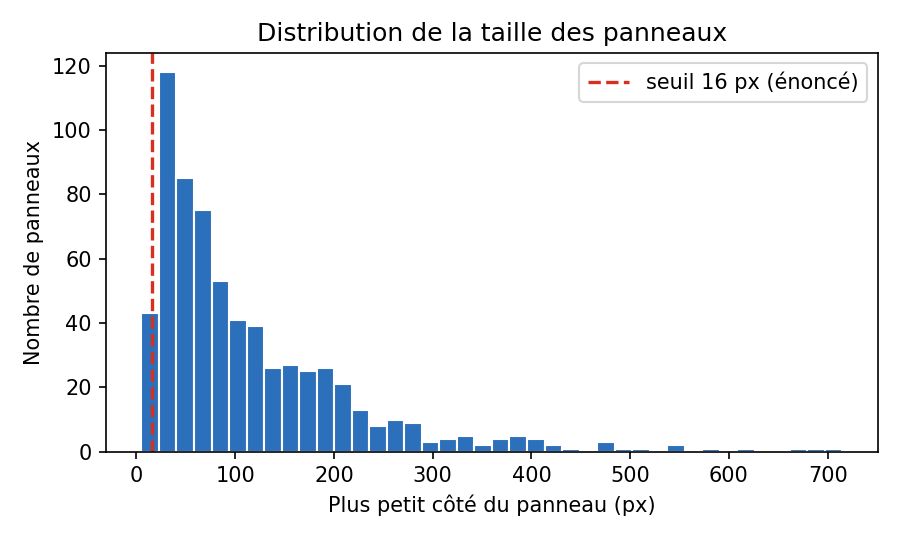
\includegraphics[width=\linewidth]{figures/dataset_tailles.png}
  \caption{Tailles}
\end{subfigure}\hfill
\begin{subfigure}{0.32\linewidth}
  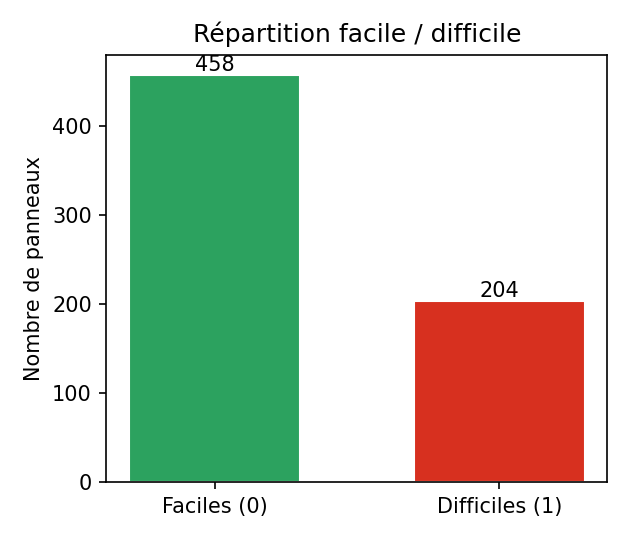
\includegraphics[width=\linewidth]{figures/dataset_difficulte.png}
  \caption{Difficulté}
\end{subfigure}\hfill
\begin{subfigure}{0.32\linewidth}
  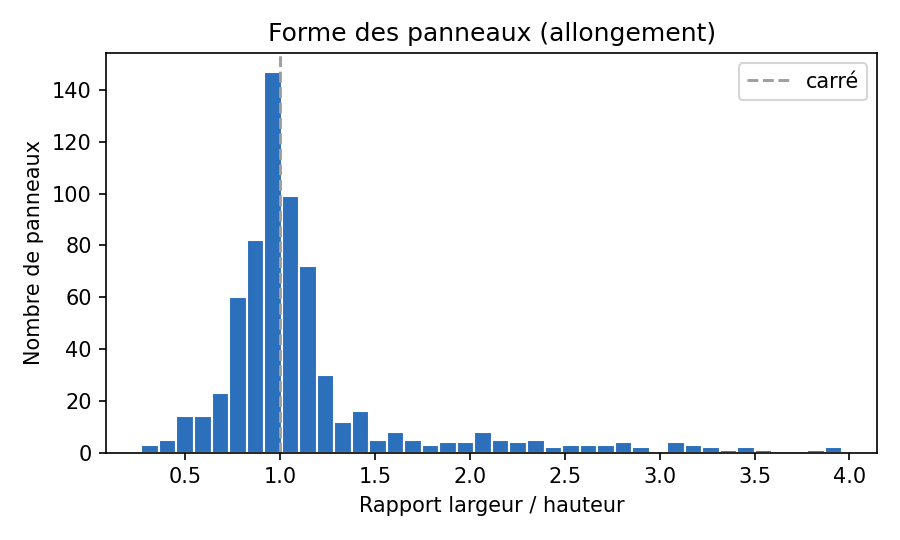
\includegraphics[width=\linewidth]{figures/dataset_formes.png}
  \caption{Forme}
\end{subfigure}
\caption{Statistiques du jeu de données annoté (341 images, 662 boîtes).}
\label{fig:dataset}
\end{figure}

\textbf{La correction de la base.} En relisant les annotations, nous avons repéré et
traité quelques anomalies : une boîte de taille nulle (fichier \texttt{0309}), des
boîtes dont le plus petit côté fait moins de 16~px (que l'énoncé dit de ne pas
annoter), et un déséquilibre du champ difficulté. Par sécurité, notre code
d'évaluation ignore de lui-même les boîtes de surface nulle.

\textbf{Comment on a évalué.} Le jeu de test n'ayant pas d'annotations, on ne peut
pas y calculer nos scores nous-mêmes. Nous avons donc mis de côté une partie des
images d'entraînement pour en faire un jeu de \emph{validation}. Le partage se fait
\emph{par image} et non par fenêtre : toutes les fenêtres d'une image de validation
sont donc totalement inconnues du modèle ; sinon, des bouts d'une même image se
retrouveraient des deux côtés et le score serait trompeusement bon.

Notre travail s'est déroulé en deux phases, avec deux jeux de validation différents
(ils ne sont donc pas comparables entre eux) :
\begin{itemize}[noitemsep,topsep=2pt]
\item \textbf{Phase 1} : ancien partage, \textbf{273~images} d'entraînement /
\textbf{68}~de validation. C'est là qu'on a obtenu les gros gains (découpage, hard
negatives).
\item \textbf{Phase 2} : après nettoyage et re-téléchargement de la base, nouveau
partage \textbf{329~/~12}. Validation plus petite (donc AP plus bruitée, à lire avec
prudence), utilisée pour régler le filtre couleur et la texture.
\end{itemize}

\textit{Remarque pour la livraison.} Pour le rendu final, les images de validation
sont réintégrées à l'entraînement afin que le modèle livré apprenne sur \emph{toutes}
les données. Les chiffres présentés ici restent ceux de la validation, c'est là qu'on
a jugé chaque idée.

% ----------------------------------------------------------------------
\section{Comment fonctionne notre détecteur}
% ----------------------------------------------------------------------
Notre programme est organisé en plusieurs fichiers Python (un par rôle) : chargement
des données, calcul des descripteurs, entraînement, détection, métriques, et des
scripts qui orchestrent le tout. Voici la chaîne complète, dans l'ordre.

\subsection{Préparer les exemples}
Le classifieur a besoin d'exemples « panneau » et « pas panneau », tous de même
taille.
\begin{itemize}[noitemsep,topsep=2pt]
\item \textbf{Exemples positifs} : pour chaque boîte annotée, on découpe le panneau
dans l'image. Comme les panneaux ne sont pas tous carrés, on agrandit le côté le plus
court en prenant du \emph{vrai contexte} autour (pas des bandes noires), puis on
redimensionne le tout en \textbf{$64\times64$ pixels}.
\item \textbf{Exemples négatifs} : on prend au hasard des morceaux d'images
\emph{sans} panneau (10 morceaux par image), eux aussi ramenés en $64\times64$.
\end{itemize}

\subsection{Décrire une imagette : forme + couleur + texture}
Une imagette $64\times64$ n'est pas donnée telle quelle au classifieur : on la résume
par un \emph{descripteur}, c'est-à-dire une liste de nombres qui capture l'essentiel.
\begin{itemize}[noitemsep,topsep=2pt]
\item \textbf{HOG} (histogramme de gradients orientés, 1764 valeurs) : il mesure, par
petites zones, dans quelles directions les contours sont marqués. Il décrit donc la
\emph{forme} (cercle, triangle, etc.).
\item \textbf{Histogramme de couleur HSV} (84 valeurs) : il résume les couleurs
présentes. Utile car les panneaux ont des couleurs typiques (rouge, bleu, jaune).
\item \textbf{Histogramme de texture LBP} (\emph{Local Binary Pattern}, 10 valeurs) :
il décrit la régularité locale de la surface, pour aider à séparer un panneau lisse
d'un fond texturé (feuillage, brique).
\end{itemize}
Les trois descripteurs sont mis bout à bout en un seul vecteur de \textbf{1858
nombres}. C'est ce vecteur qui représente l'imagette.

\subsection{Entraîner le classifieur, puis le corriger (hard negative mining)}
Le classifieur est un \textbf{Random Forest} (« forêt aléatoire ») : un ensemble de
100~arbres de décision qui votent ; la proportion de votes « panneau » donne un score
entre 0 et 1.

L'entraînement se fait en deux temps :
\begin{enumerate}[noitemsep,topsep=2pt]
\item \textbf{Premier entraînement} sur les positifs et les négatifs décrits ci-dessus.
\item \textbf{Hard negative mining} : on fait passer le modèle sur beaucoup de
morceaux d'images \emph{sans} panneau, à plusieurs tailles. Tous ceux qu'il prend à
tort pour des panneaux sont ses « erreurs » ; on les rajoute aux négatifs et on
réentraîne. Le modèle apprend ainsi à ne plus se faire piéger par ces fonds
trompeurs. Cette étape est rapide car on évalue tous les morceaux d'un coup.
\end{enumerate}

\subsection{Détecter sur une image entière}
Pour une nouvelle image, on cherche les panneaux ainsi :
\begin{enumerate}[noitemsep,topsep=2pt]
\item \textbf{Pré-filtrage couleur} : on construit un masque des pixels « couleur
panneau » (rouge, bleu ou jaune saturés) et, grâce à une \emph{image intégrale}, on
ne lancera le classifieur que sur les fenêtres assez colorées. Cela écarte d'emblée le
ciel, la route ou les façades grises, ce qui accélère et réduit les fausses
détections. Un garde-fou désactive le filtre pour les images très sombres (scènes de
nuit), où les couleurs sont peu saturées, afin de ne pas rater ces panneaux.
\item \textbf{Pyramide d'images} : on regarde l'image à sa taille normale, puis de
plus en plus réduite (chaque niveau est $1{,}25$ fois plus petit). Comme la fenêtre de
recherche garde une taille fixe ($64\times64$), réduire l'image revient à chercher des
panneaux de plus en plus grands.
\item \textbf{Fenêtre glissante} : à chaque niveau, une fenêtre $64\times64$ se
déplace par pas de 16~pixels. Chaque position retenue donne une imagette, qu'on décrit
(HOG + couleur + texture) et qu'on classe.
\item \textbf{Score et seuil} : pour l'\emph{évaluation}, on garde un seuil bas
($0{,}3$) afin de tracer toute la courbe de performance ; pour la \emph{soumission},
on relève ce seuil pour ne garder que les détections sûres (voir
section~\ref{sec:soumission}).
\item \textbf{Remise à l'échelle} : les positions trouvées sur une image réduite sont
ramenées aux coordonnées de l'image d'origine.
\end{enumerate}

\subsection{Nettoyer les boîtes en double (NMS)}
\label{sec:nms}
La fenêtre glissante détecte souvent le même panneau plusieurs fois. La
\textbf{suppression des non-maxima} (NMS) garde, parmi des boîtes qui se chevauchent,
celle au meilleur score et supprime les autres. Deux boîtes sont jugées « en double »
si elles se recouvrent beaucoup (IoU élevé) \emph{ou} si l'une est largement contenue
dans l'autre. Ce second critère corrige un défaut de la NMS classique : une petite
boîte à l'intérieur d'une grande a un IoU très faible et passerait donc à travers
(détaillé en section~\ref{sec:exp}).

\subsection{Sauvegarder le modèle et produire le fichier de test}
Entraîner prend du temps ; on ne veut pas recommencer à chaque détection. Une fois le
modèle prêt, on l'enregistre dans \texttt{modele\_panneaux.joblib} (bibliothèque
\texttt{joblib}). Le script de prédiction recharge ce fichier au lieu de tout refaire ;
une option \texttt{retrain} force un nouvel entraînement quand le code a changé. Ce
fichier de modèle fait partie des livrables demandés.

Le script de test parcourt ensuite toutes les images du dossier \texttt{test/},
applique la détection puis la NMS, et écrit un seul fichier \texttt{detection.csv} au
format exigé : \texttt{Num img, ymin, xmin, hauteur, largeur, score}, une ligne par
détection.

\subsection{Récapitulatif des paramètres}
\begin{table}[h]
\centering
\caption{Principaux paramètres de la chaîne.}
\begin{tabular}{ll}
\toprule
Paramètre & Valeur \\
\midrule
Taille des imagettes                & $64\times64$ px \\
Pas de la fenêtre glissante         & 16 px \\
Réduction entre niveaux de pyramide & $\times 1{,}25$ \\
Seuil de score (évaluation)         & 0{,}3 \\
Seuil de score (soumission)         & 0{,}6 \\
Seuil d'IoU pour la NMS             & 0{,}3 \\
Seuil d'IoU vérité/détection        & 0{,}5 \\
Pré-filtre couleur (fraction min.)  & 0{,}05 \\
Négatifs aléatoires par image       & 10 \\
Tailles des morceaux (hard neg.)    & 64, 96, 128, 200, 300 px \\
Random Forest                       & 100 arbres \\
Descripteur HOG                     & 9 orientations, cellules $8\times8$, blocs $2\times2$ \\
Descripteur couleur                 & histogramme HSV (36+32+16) \\
Descripteur texture                 & histogramme LBP uniform (P=8, R=1) \\
Taille du vecteur final             & 1858 \\
\bottomrule
\end{tabular}
\label{tab:params}
\end{table}

% ----------------------------------------------------------------------
\section{Comment on mesure la performance}
\label{sec:metriques}
% ----------------------------------------------------------------------
Pour décider si une idée est bonne, il faut un chiffre fiable. Nous avons codé nos
propres métriques (fichier \texttt{metrics.py}).

\textbf{IoU (recouvrement de deux boîtes).} On compare une boîte trouvée à une vraie
boîte en regardant la surface commune divisée par la surface totale :
\begin{equation}
\mathrm{IoU}(A,B) = \frac{\mathrm{aire}(A \cap B)}{\mathrm{aire}(A \cup B)} .
\end{equation}
Une détection est juste (un \emph{vrai positif}) si son IoU avec une vraie boîte non
encore prise est $\geq 0{,}5$ ; sinon c'est une fausse détection. Une même vraie boîte
ne peut être comptée qu'une fois.

\textbf{Précision et rappel.} La \emph{précision} dit « parmi ce que j'ai détecté,
quelle part est correcte » ; le \emph{rappel} dit « parmi les vrais panneaux, combien
j'ai retrouvés » :
\begin{equation}
\text{Précision} = \frac{VP}{VP + FP}, \qquad
\text{Rappel} = \frac{VP}{VP + FN}.
\end{equation}

\textbf{AP (aire sous la courbe précision/rappel).} En classant toutes les détections
du score le plus haut au plus bas, précision et rappel évoluent : on obtient une
courbe (figure~\ref{fig:pr}), et l'\emph{Average Precision} en est l'aire. C'est notre
note principale. Nous rapportons aussi le \textbf{F1} (compromis entre précision et
rappel) ainsi que la précision et le rappel au point où le F1 est le meilleur.

\begin{figure}[h]
\centering
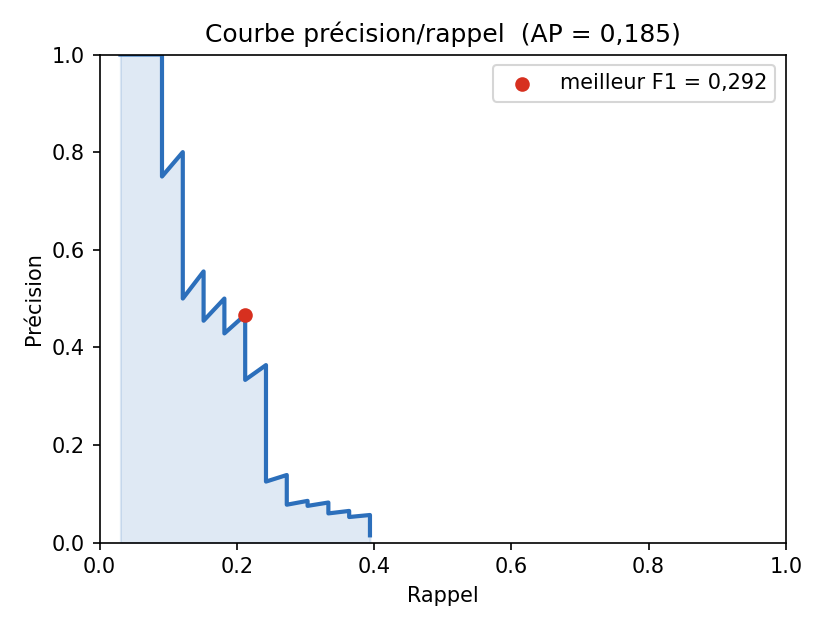
\includegraphics[width=0.55\linewidth]{figures/courbe_pr.png}
\caption{Courbe précision/rappel du détecteur final sur la validation. Le point rouge
marque le meilleur F1. L'aire sous la courbe est l'AP.}
\label{fig:pr}
\end{figure}

\textbf{Deux seuils différents (à ne pas confondre).} Le \emph{seuil de score} décide
quelles détections on garde selon la confiance du modèle ; il ne change rien à
l'entraînement. Le \emph{seuil d'IoU} mesure un recouvrement géométrique : 0{,}3 dans
la NMS (repérer les doublons) et 0{,}5 pour décider si une détection tombe bien sur un
vrai panneau.

% ----------------------------------------------------------------------
\section{Notre progression, étape par étape}
\label{sec:exp}
% ----------------------------------------------------------------------

\subsection{Le point de départ : un piège}
La toute première chaîne obtenait \textbf{98{,}96\,\% de bonnes réponses} quand on lui
donnait des imagettes déjà découpées... mais seulement \textbf{AP $=0{,}095$} en vraie
détection. L'explication : bien classer une imagette déjà centrée est facile, mais sur
une image entière on teste des milliers de fenêtres, et même 1\,\% d'erreur fait
apparaître des milliers de fausses boîtes. \emph{Leçon : le score sur imagettes est
trompeur ; seule la détection sur image entière compte.} C'est ce constat qui a
justifié toute la suite.

\subsection{Mieux découper les exemples positifs}
Au départ, les panneaux non carrés étaient complétés par des \emph{bandes noires} pour
devenir carrés. Le HOG apprenait alors ces bords noirs, qui n'existent jamais dans une
vraie fenêtre. En les remplaçant par du vrai contexte de l'image, l'AP monte de
\textbf{0{,}095 à 0{,}173} ($+82\,\%$). Premier vrai gain.

\subsection{Apprendre de ses erreurs : hard negative mining}
Le détecteur voyait des panneaux partout. En lui réinjectant ses fausses détections
comme contre-exemples, l'AP grimpe de \textbf{0{,}173 à 0{,}293} ($+69\,\%$), et le
nombre de détections \emph{baisse} de 19\,341 à 11\,039 : il se trompe beaucoup moins.
La figure~\ref{fig:progression} et le tableau~\ref{tab:progression} résument cette
progression.

\begin{figure}[h]
\centering
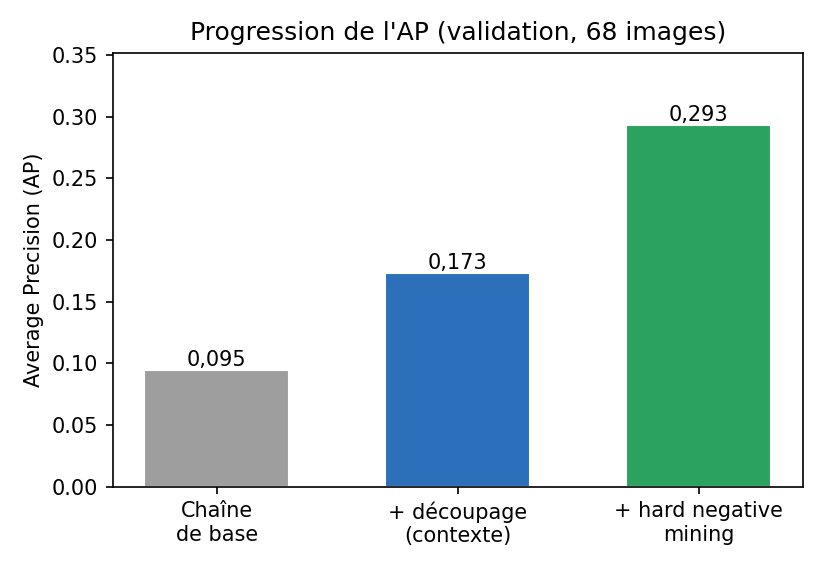
\includegraphics[width=0.52\linewidth]{figures/ap_progression.png}
\caption{Évolution de l'AP au fil des deux grandes améliorations (phase 1, 68 images).}
\label{fig:progression}
\end{figure}

\begin{table}[h]
\centering
\caption{Progression sur la validation (phase 1 : 68 images, 147 panneaux).}
\begin{tabular}{lccc}
\toprule
Étape & AP & $F_1$ & Détections \\
\midrule
Chaîne de base                   & 0,095 & 0,224 & 8\,511 \\
\;+ meilleur découpage (contexte) & 0,173 & 0,272 & 19\,341 \\
\;+ hard negative mining          & \textbf{0,293} & \textbf{0,387} & 11\,039 \\
\bottomrule
\end{tabular}
\label{tab:progression}
\end{table}

\subsection{Couleur et texture : pré-filtre + LBP}
Sur le jeu nettoyé (phase 2, 12 images), nous avons ajouté le \emph{pré-filtrage
couleur} puis le descripteur de \emph{texture LBP}. Le pré-filtre couleur ne change
quasiment pas l'AP mais réduit fortement le nombre de fausses détections et le temps de
calcul (jusqu'à $\approx 4\times$ plus rapide en version stricte). Le LBP, lui, fait
remonter l'AP et le rappel ensemble (tableau~\ref{tab:ablation},
figure~\ref{fig:ablation}) : il aide réellement à distinguer un panneau d'un fond
texturé. \emph{Réserve honnête} : ces écarts sont mesurés sur seulement 12 images,
donc bruités ; ils indiquent une tendance, pas une preuve définitive.

\begin{figure}[h]
\centering
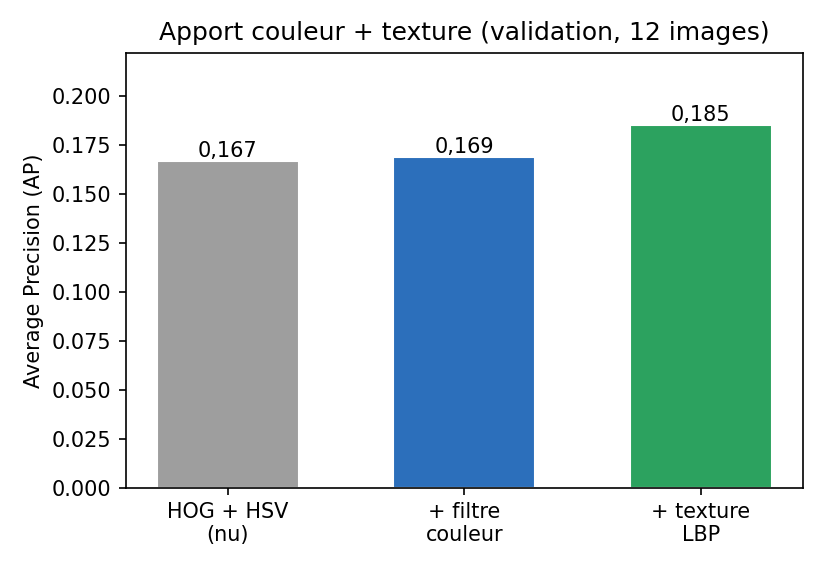
\includegraphics[width=0.52\linewidth]{figures/ablation_descripteurs.png}
\caption{Apport du filtre couleur puis du LBP (phase 2, validation 12 images).}
\label{fig:ablation}
\end{figure}

\begin{table}[h]
\centering
\caption{Ablation des descripteurs (phase 2 : 12 images, 33 panneaux).}
\begin{tabular}{lcccc}
\toprule
Configuration & AP & $F_1$ & Rappel & Détections \\
\midrule
HOG + HSV (nu)        & 0,167 & 0,273 & 0,182 & 1\,218 \\
\;+ filtre couleur     & 0,169 & 0,273 & 0,182 & 1\,042 \\
\;+ texture LBP        & \textbf{0,185} & \textbf{0,292} & \textbf{0,212} & 877 \\
\bottomrule
\end{tabular}
\label{tab:ablation}
\end{table}

\subsection{Nettoyer les boîtes imbriquées (NMS)}
En regardant les détections, on voyait plusieurs boîtes empilées sur un même panneau.
La NMS classique ne les supprimait pas car une petite boîte dans une grande a un IoU
minuscule (par exemple $64\times64$ dans $305\times305$ donne un IoU d'environ
$0{,}04$). Nous avons donc ajouté le critère de « contenance ». Une variante qui
gardait la \emph{plus grande} boîte a été essayée puis abandonnée : une grosse boîte
parasite couvrant plusieurs panneaux les faisait tous disparaître. On garde donc la
boîte \emph{la plus confiante}.

\subsection{Random Forest contre SVM}
Nous avons comparé, sur les mêmes 25~images, le Random Forest et un \textbf{SVM
linéaire} (descripteurs mis à l'échelle et scores ramenés entre 0 et 1 pour une
comparaison juste). Le Random Forest gagne largement (tableau~\ref{tab:rfsvm},
figure~\ref{fig:rfsvm}) : le SVM linéaire sépare moins bien nos descripteurs, là où la
forêt combine mieux les indices de forme, de couleur et de texture. \textbf{Nous
gardons le Random Forest.}

\begin{figure}[h]
\centering
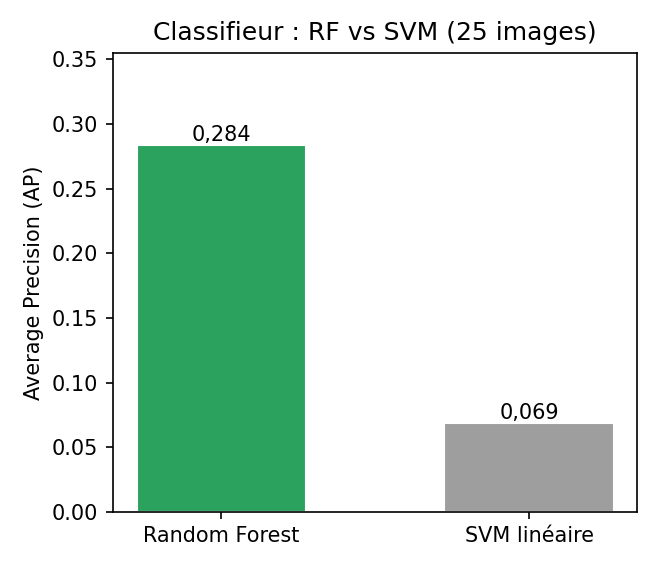
\includegraphics[width=0.42\linewidth]{figures/rf_vs_svm.png}
\caption{Random Forest contre SVM linéaire (mêmes 25 images).}
\label{fig:rfsvm}
\end{figure}

\begin{table}[h]
\centering
\caption{Random Forest contre SVM linéaire (mêmes 25 images).}
\begin{tabular}{lccc}
\toprule
Modèle & AP & $F_1$ & Rappel (détection) \\
\midrule
Random Forest   & \textbf{0,284} & \textbf{0,429} & --- \\
SVM linéaire     & 0,069 & 0,194 & 0,149 \\
\bottomrule
\end{tabular}
\label{tab:rfsvm}
\end{table}

\subsection{Préparer le fisheye par augmentation (essai non retenu)}
Comme on ne peut pas savoir quelles images de test seront fisheye, nous avons préféré
\emph{apprendre} des panneaux déformés plutôt que de corriger les images au test. Nous
avons donc ajouté une version déformée (effet « grand-angle ») de chaque panneau
positif. Faute d'images fisheye en validation, le garde-fou était : « est-ce que ça
casse le cas normal ? ». Réponse : oui, l'AP tombe de $0{,}284$ à $0{,}221$ sur
25~images, et réduire la déformation n'y change rien. La raison : on double le nombre
de positifs, ce qui déséquilibre les exemples. Nous avons donc \textbf{désactivé}
cette augmentation (le code reste disponible).

\subsection{S'attaquer aux panneaux triangulaires (essai non concluant)}
Sur les triangles, le modèle donnait parfois plus de confiance à une petite boîte
posée sur un \emph{coin} (deux arêtes nettes) qu'à la boîte cadrant tout le panneau.
Nous avons tenté de récupérer ces coins comme contre-exemples. Mal réglé, cela
étiquetait aussi des boîtes presque correctes en « pas panneau », et la détection
s'effondrait. Même après réglage, le résultat n'était pas convaincant : approche
\textbf{abandonnée} pour l'instant, mais conservée et documentée car elle éclaire le
vrai problème (section~\ref{sec:analyse}).

% ----------------------------------------------------------------------
\section{Soumission sur le serveur d'évaluation}
\label{sec:soumission}
% ----------------------------------------------------------------------
La détection sur les vraies images de test produit le fichier \texttt{detection.csv}
soumis sur la page web de l'UTC. Notre première soumission (seuil de score $0{,}3$)
donne un \textbf{rappel correct ($\approx 31\,\%$)} mais une \textbf{précision
minuscule ($\approx 0{,}8\,\%$)}, d'où un F1 et une AUC plombés.

\textbf{Diagnostic.} Une précision de $0{,}8\,\%$ veut dire que, pour 100 boîtes
écrites dans le fichier, environ 99 sont fausses. Le coupable n'est pas le modèle en
lui-même mais le \emph{seuil de score} : nous l'avions laissé bas ($0{,}3$) — utile
pour tracer la courbe AP, mais désastreux pour une soumission, car il laisse passer
des milliers de fenêtres faiblement notées. C'est la version « image entière » du même
piège qu'au tout début : un classifieur correct, noyé sous les fausses alarmes dès
qu'on garde tout.

\textbf{Correction.} Pour la soumission, on relève le seuil de score à \textbf{0{,}6} :
on ne garde que les détections sûres. L'effet, mesuré par une seconde soumission, est
spectaculaire (figure~\ref{fig:soumission} et tableau~\ref{tab:soumission}) : la
précision est multipliée par~18 ($0{,}8 \to 15{,}2\,\%$), le rappel ne perd presque
rien ($31 \to 26{,}9\,\%$), et le F1 comme l'AUC progressent fortement (F1
$1{,}6 \to 19{,}4\,\%$, AUC $18{,}6 \to 23{,}7\,\%$). Le fichier passe de 385~ko à
18~ko. C'est un simple réglage de \emph{point de fonctionnement}, sans
réentraînement : le défaut dominant était bien le seuil, pas le modèle.

\begin{figure}[h]
\centering
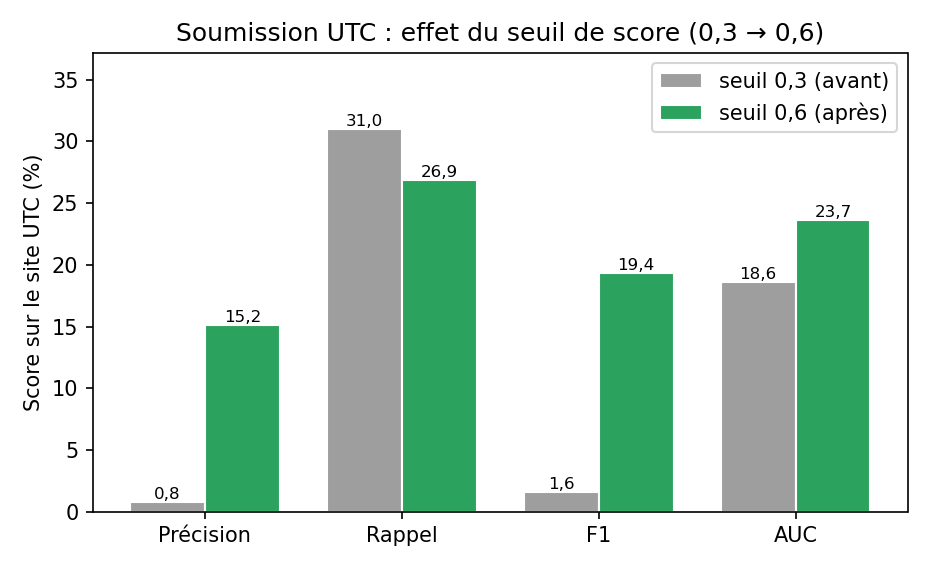
\includegraphics[width=0.62\linewidth]{figures/soumission_utc.png}
\caption{Soumissions UTC avant/après le relèvement du seuil de score. À seuil bas la
précision s'effondre ; à $0{,}6$ elle remonte fortement sans presque perdre de rappel.}
\label{fig:soumission}
\end{figure}

\begin{table}[h]
\centering
\caption{Effet du seuil de score sur la soumission UTC (scores du site, en \%).}
\begin{tabular}{lcccc}
\toprule
Soumission & Précision & Rappel & $F_1$ & AUC \\
\midrule
Seuil 0,3 (avant) & 0,82 & \textbf{30,97} & 1,59 & 18,59 \\
Seuil 0,6 (après) & \textbf{15,16} & 26,87 & \textbf{19,38} & \textbf{23,68} \\
\bottomrule
\end{tabular}
\label{tab:soumission}
\end{table}

% ----------------------------------------------------------------------
\section{Analyse : quand ça marche, quand ça coince}
\label{sec:analyse}
% ----------------------------------------------------------------------
\textbf{Ce qui marche bien.} Les panneaux nets, de taille moyenne à grande et bien
colorés (rouge ou bleu sur fond clair) sont bien détectés et bien notés.

\textbf{Ce qui coince.}
\begin{itemize}[noitemsep,topsep=2pt]
\item \emph{Excès de fausses détections} à bas seuil : c'est le défaut dominant
(section~\ref{sec:soumission}), maîtrisé en relevant le seuil de soumission.
\item \emph{Panneaux triangulaires} : le modèle peut préférer un coin du triangle au
panneau entier. Le souci n'est pas la NMS mais le classifieur, qui note la présence de
« texture de panneau » sans tenir compte du bon cadrage.
\item \emph{Boîtes avec trop de fond} : certaines détections contiennent plus
d'arrière-plan que de panneau, signe que le modèle s'appuie trop sur le décor.
\item \emph{Petits panneaux lointains} : plus difficiles à trouver et à cadrer, à
cause de la taille minimale de fenêtre et du pas.
\item \emph{Fisheye} : pas mesurable chez nous (aucune image fisheye en validation),
donc robustesse incertaine.
\end{itemize}

\textbf{Illustration qualitative.} Le dossier \texttt{images\_results/} contient les
images de test annotées (boîtes + scores) produites à chaque lancement. La
figure~\ref{fig:qualitatif} en montre un cas réussi et un cas d'échec typique.

\begin{figure}[h]
\centering
\begin{subfigure}{0.46\linewidth}
  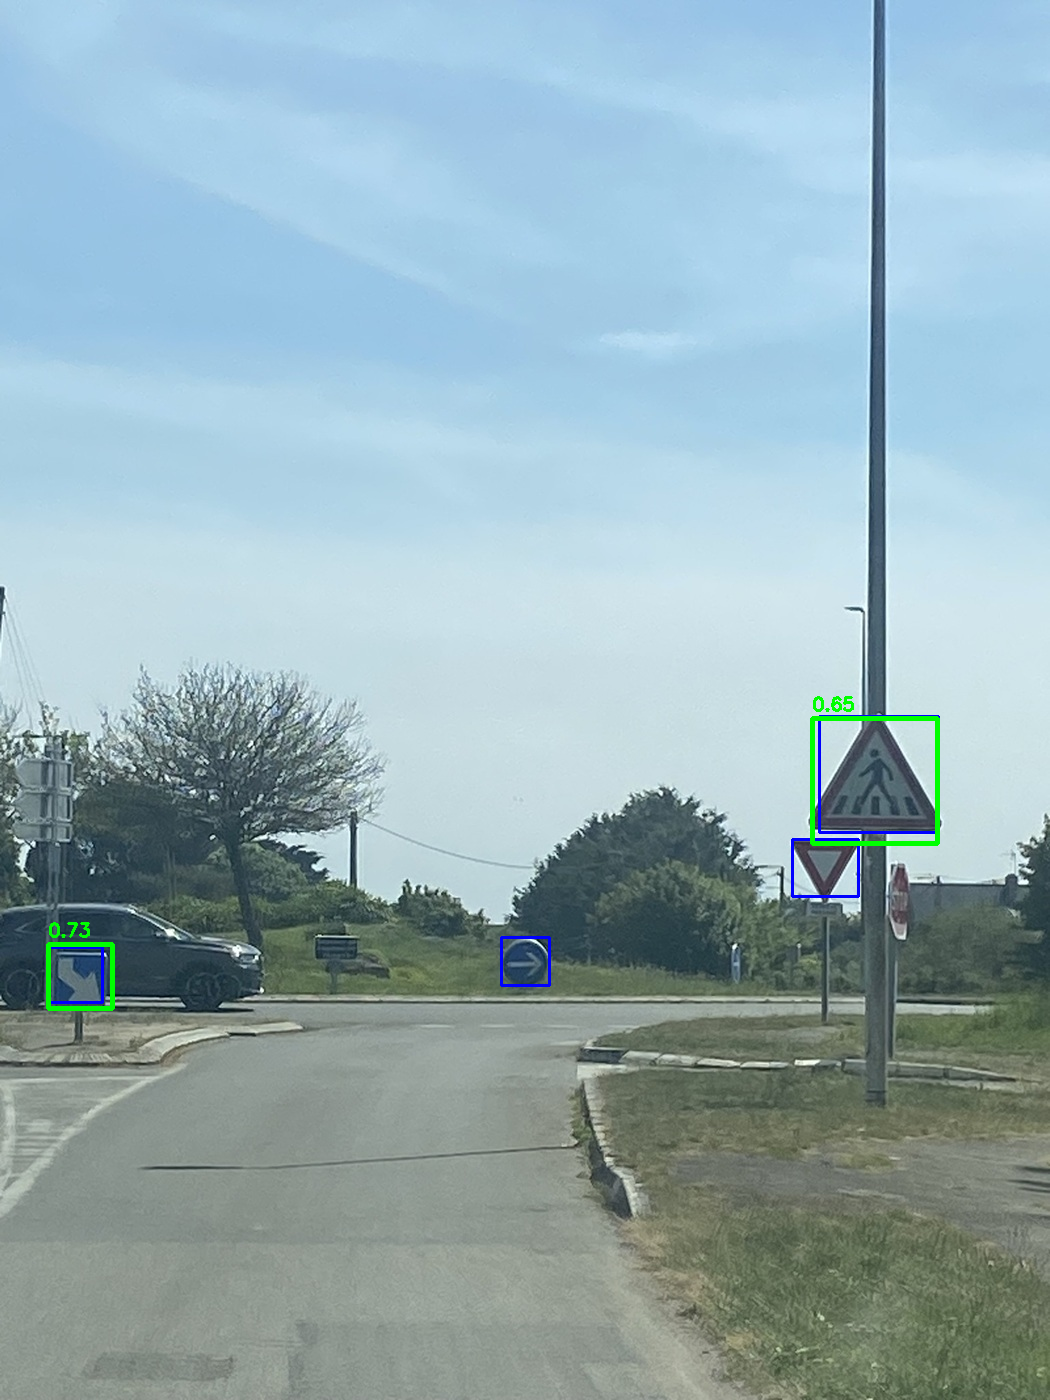
\includegraphics[width=\linewidth]{figures/exemple_reussite.png}
  \caption{Réussite : panneau bien cadré et bien noté.}
\end{subfigure}\hfill
\begin{subfigure}{0.46\linewidth}
  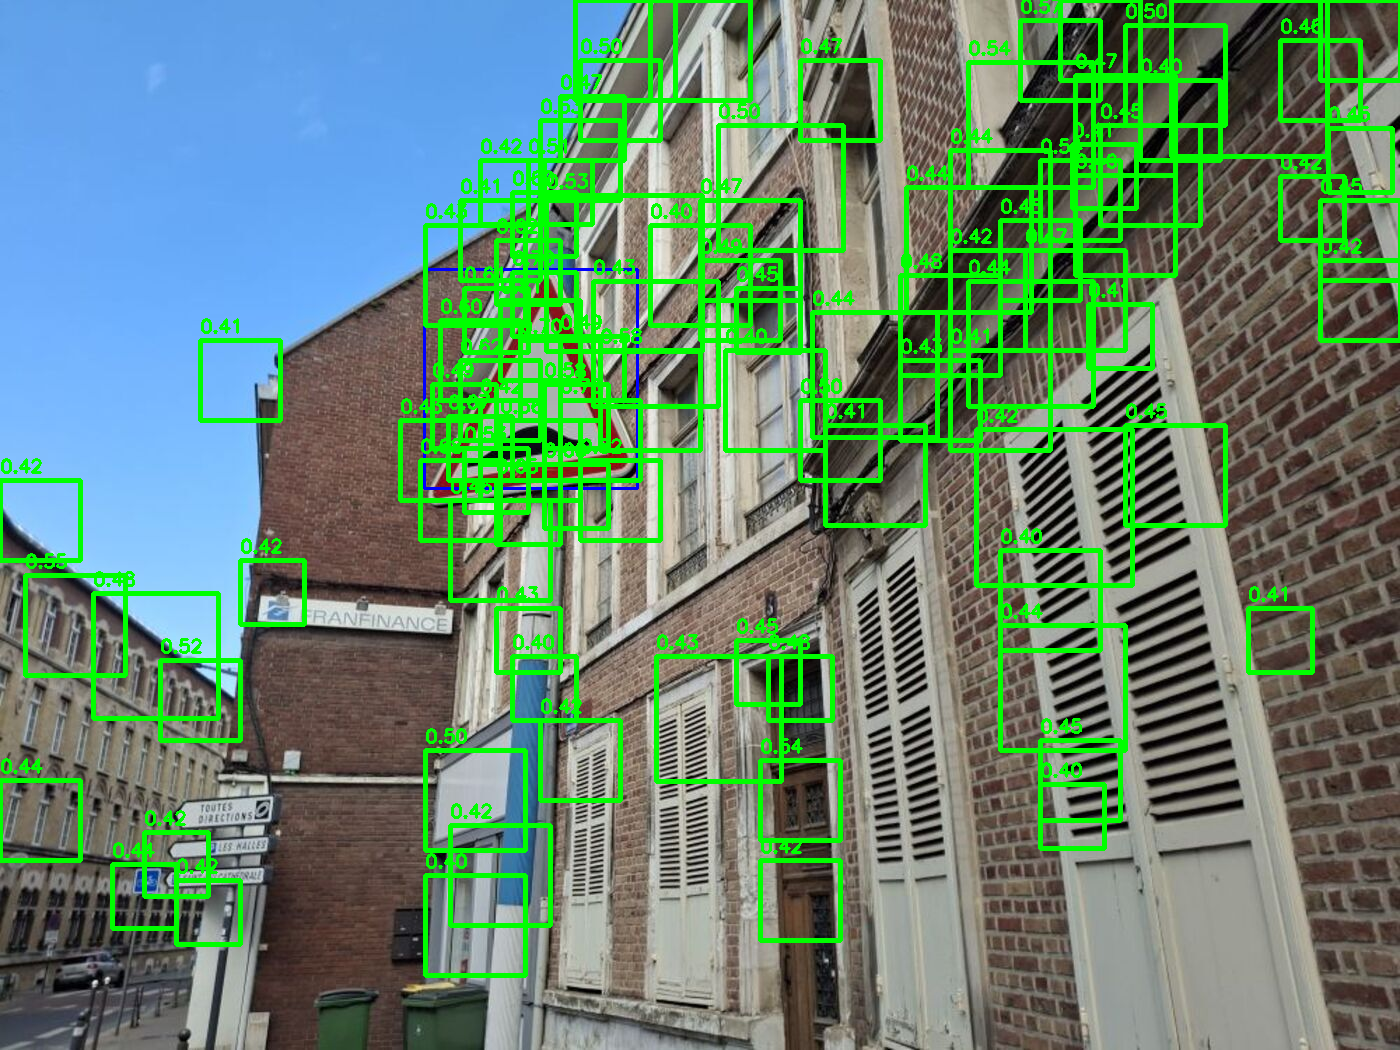
\includegraphics[width=\linewidth]{figures/exemple_echec.png}
  \caption{Échec : sur-détection / boîte mal cadrée.}
\end{subfigure}
\caption{Exemples qualitatifs (à choisir dans \texttt{images\_results/} et copier dans
\texttt{figures/}).}
\label{fig:qualitatif}
\end{figure}

\textbf{Temps de calcul.} L'étape lente est la fenêtre glissante : environ 130~s par
image avec un pas de 5~px, ramené à $\approx 13$~s avec un pas de 16~px, la prédiction
répartie sur tous les cœurs et le pré-filtre couleur. La NMS ralentit aussi quand les
détections sont très nombreuses (complexité en $O(n^2)$).

% ----------------------------------------------------------------------
\section{Conclusion et perspectives}
% ----------------------------------------------------------------------
En suivant notre fil conducteur — d'abord mesurer, ensuite améliorer — nous avons fait
passer l'AP de $0{,}095$ à $0{,}293$ sur la validation, principalement grâce à un
meilleur découpage des exemples et au hard negative mining ; la couleur et la texture
apportent un gain supplémentaire. Tout aussi instructif : nous avons \emph{écarté} sur
preuve plusieurs idées (augmentation fisheye trop forte, hard negatives ciblés mal
réglés, SVM linéaire), ce qui montre l'intérêt d'une évaluation rigoureuse. La
première soumission a enfin révélé un défaut de précision lié au seuil de score :
en le relevant à $0{,}6$, l'AUC du serveur passe de $18{,}6$ à $23{,}7\,\%$ et le F1
de $1{,}6$ à $19{,}4\,\%$.

La prochaine priorité est d'aider le classifieur à mieux « faire confiance » aux
boîtes bien cadrées plutôt qu'aux sous-régions ou aux boîtes pleines de fond :
enrichir les exemples positifs, plafonner le nombre de détections gardées par image,
et calibrer les scores. Ces pistes devraient notamment aider sur les panneaux
triangulaires et faire encore monter la précision en soumission.

% ----------------------------------------------------------------------
\section*{Déclaration d'utilisation d'IA générative}
% ----------------------------------------------------------------------
\addcontentsline{toc}{section}{Déclaration IA générative}
Conformément à l'énoncé, nous déclarons avoir utilisé un assistant d'IA générative
pour : la mise en place des
métriques et du protocole d'évaluation, l'aide au débogage, la génération des figures,
et la rédaction de ce rapport. Exemples de requêtes employées :
\begin{itemize}[noitemsep,topsep=2pt]
\item « Implémente les métriques de détection (IoU, précision/rappel, AP, F1) en code
simple et commenté. »
\item « Pourquoi mon AP est-elle faible alors que le score sur imagettes est de 99\,\% ? »
\item « Rends le hard negative mining multi-échelle. »
\item « Pourquoi ma précision est-elle de 0{,}8\,\% en soumission, et comment la corriger ? »
\end{itemize}
Toutes les décisions, mesures et validations ont été contrôlées par les auteurs.

% ----------------------------------------------------------------------
\section*{Contributions}
% ----------------------------------------------------------------------
\addcontentsline{toc}{section}{Contributions}
Projet réalisé en binôme dans le cadre de l'UE SY32 (P2026) à l'UTC.
Conception, implémentation, évaluation et rédaction ont été menées conjointement.

\end{document}
